%% retrank @ NTCIR-19 R2C2 --- oral presentation
%% SLOT: Wed 9 Dec 2026, 13:20-14:20 session, Room 2. retrank is 4th of 4 teams (~14:03).
%% BUDGET: 12 min total = 10 min talk + 2 min Q&A.
%% Pacing target below is ~10:00. Timings are in the \note{} on each slide.
\documentclass[aspectratio=169,11pt]{beamer}
\usetheme{default}
\usepackage[utf8]{inputenc}
\usepackage[T1]{fontenc}
\usepackage{booktabs}
\usepackage{amsmath}
\usepackage{tikz}
\usetikzlibrary{positioning,arrows.meta}

\definecolor{ink}{HTML}{14213D}
\definecolor{accent}{HTML}{BC4749}
\definecolor{good}{HTML}{2A6F4E}
\definecolor{panel}{HTML}{F2F3F5}
\definecolor{rule}{HTML}{C8CCD4}

\setbeamercolor{frametitle}{fg=white,bg=ink}
\setbeamercolor{title}{fg=ink}
\setbeamercolor{structure}{fg=ink}
\setbeamercolor{block title}{fg=white,bg=ink}
\setbeamercolor{block body}{bg=panel}
\setbeamertemplate{navigation symbols}{}
\setbeamertemplate{itemize item}{\color{ink}$\blacktriangleright$}
\setbeamertemplate{footline}{\hfill\tiny\color{gray}
  retrank\;\textbar\;NTCIR-19 R2C2\quad\insertframenumber/\inserttotalframenumber\quad}
\setbeamerfont{frametitle}{size=\large,series=\bfseries}

\newcommand{\HMR}{\textsc{HMR}}
\newcommand{\MNP}{\textsc{MNP}}
\newcommand{\RO}{R_{\mathrm{O}}}
\newcommand{\RU}{R_{\mathrm{U}}}
\newcommand{\hl}[1]{{\color{accent}\textbf{#1}}}
\newcommand{\gd}[1]{{\color{good}\textbf{#1}}}

\title{Answering with Confidence is a Calibration Problem}
\subtitle{retrank at the NTCIR-19 R2C2 Task}
\author{Alessandro Magnani}
\institute{Independent Researcher}
\date{NTCIR-19 \textbar\ Tokyo \textbar\ 9 December 2026}

\begin{document}

%% ---------------------------------------------------------------- 0:00 -- 0:20
\begin{frame}[plain]
  \titlepage
\end{frame}
\note{0:20 cumulative. Say the title sentence and move -- do not linger.}

%% ---------------------------------------------------------------- 0:20 -- 1:20
\begin{frame}{\HMR{} is not a QA metric}
\begin{columns}[T]
\begin{column}{0.56\textwidth}
\begin{itemize}\setlength\itemsep{0.5em}
  \item AC asks for an answer, a \textbf{confidence} in $[0,100]$, and grounded nuggets
  \item \HMR{} rewards being confident \emph{when right} and diffident \emph{when wrong}
        --- the organisers' \emph{modesty}
  \item[] 
  \item \hl{It is a calibration metric.}
        That turned out to be most of the story.
\end{itemize}
\end{column}
\begin{column}{0.42\textwidth}
\begin{block}{Decomposition}
\[ \HMR = \mathrm{harmonic\ mean}(\RO,\RU) \]
\begin{itemize}
  \item $\RO$ --- penalises \textbf{over}confidence
  \item $\RU$ --- penalises \textbf{under}confidence
\end{itemize}
\vspace{0.3em}
Harmonic $\Rightarrow$ \hl{the smaller term dominates.}
\end{block}
\end{column}
\end{columns}
\end{frame}
\note{1:20. The whole talk hangs off this decomposition -- make sure it lands.}

%% ---------------------------------------------------------------- 1:20 -- 2:00
\begin{frame}{The result}
\centering
\vspace{0.5em}
{\fontsize{34}{40}\selectfont\bfseries\color{ink}
1st \quad 1st \quad 1st}\\[0.4em]
{\large \HMR{} 0.974 \qquad Accuracy 0.969 \qquad \MNP{} 0.840}

\vspace{1.2em}
\begin{block}{}
\centering\large
Our \textbf{four} runs took the \textbf{four highest \HMR{} scores} among
\textbf{25 runs from 7 teams}.\\[0.3em]
Next-best submitted run: \textbf{0.761}.
\end{block}

\vspace{0.5em}
{\small Several teams retrieved or answered very well --- this is a design emphasis,
not a shortcoming of the field.}
\end{frame}
\note{2:00. State it plainly, credit the field in one sentence, move on.}

%% ---------------------------------------------------------------- 2:00 -- 3:30
\begin{frame}{The thesis, in one comparison}
\centering
\vspace{0.3em}
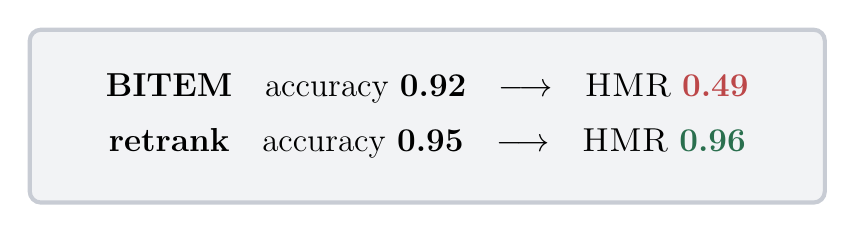
\begin{tikzpicture}[font=\large]
\node[draw=rule,fill=panel,line width=1.5pt,rounded corners,inner sep=16pt,
      text width=0.74\textwidth,align=center] {
  \textbf{BITEM}\quad accuracy \textbf{0.92}\quad$\longrightarrow$\quad\HMR{} \hl{0.49}\\[0.5em]
  \textbf{retrank}\quad accuracy \textbf{0.95}\quad$\longrightarrow$\quad\HMR{} \gd{0.96}
};
\end{tikzpicture}

\vspace{1.0em}
{\large Two systems of \textbf{comparable answer quality}. A \hl{$2\times$ gap} in \HMR.}

\vspace{0.8em}
\begin{itemize}
  \item High accuracy is \textbf{necessary but not sufficient} in R2C2
  \item What separated us was \textbf{knowing when we had answered well}
\end{itemize}
\end{frame}
\note{3:30. THE hook. Pause after the 2x. BITEM speaks before me -- acknowledge their talk here.}

%% ---------------------------------------------------------------- 3:30 -- 4:45
\begin{frame}{Most of the field collapses on one side}
\centering\vspace{0.3em}
\begin{tabular}{lccccc}
\toprule
Run & mode & conf. & acc. & $\RO$ & $\RU$\\
\midrule
\textbf{retrank-AC-1} & calibrated & 0.956 & 0.953 & \gd{0.95} & \gd{1.00}\\
ORG-AC-1 & overconfident & 0.905 & 0.531 & \hl{0.09} & 0.90\\
hit-u-AC-4 & under-confident & 0.016 & 0.813 & 0.99 & \hl{0.02}\\
\bottomrule
\end{tabular}

\vspace{1.0em}
\begin{itemize}
  \item Confident and wrong $\Rightarrow$ $\RO$ collapses
  \item Right but silent $\Rightarrow$ $\RU$ collapses
  \item \hl{Either one sinks the harmonic mean.} Keeping \emph{both} high is the task.
\end{itemize}
\end{frame}
\note{4:45. Two failure modes, one sentence each. Do not read the table aloud.}

%% ---------------------------------------------------------------- 4:45 -- 6:00
\begin{frame}{Method: answer first, then verify}
\centering\vspace{0.2em}
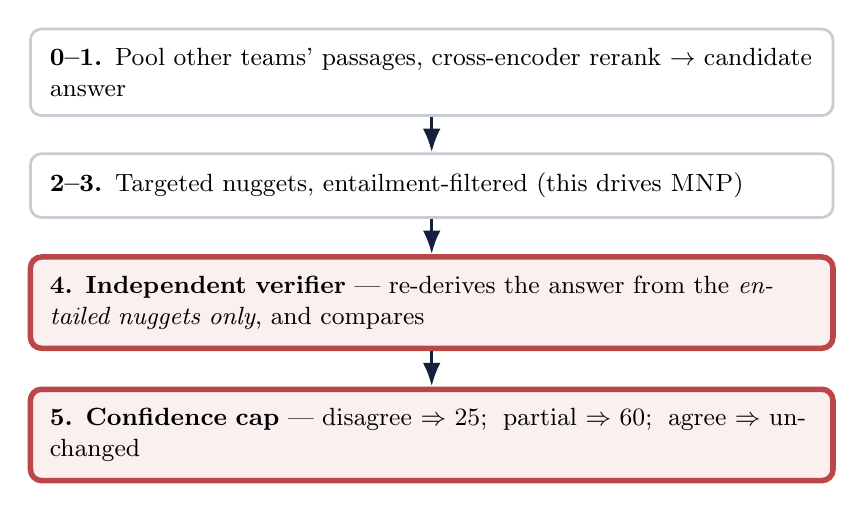
\begin{tikzpicture}[font=\small,node distance=0.45cm,
  s/.style={draw=rule,fill=white,line width=1pt,rounded corners,
            text width=0.80\textwidth,inner sep=7pt},
  k/.style={draw=accent,fill=accent!8,line width=2pt,rounded corners,
            text width=0.80\textwidth,inner sep=7pt}]
\node[s] (a) {\textbf{0--1.} Pool other teams' passages, cross-encoder rerank $\to$ candidate answer};
\node[s,below=of a] (b) {\textbf{2--3.} Targeted nuggets, entailment-filtered (this drives \MNP)};
\node[k,below=of b] (c) {\textbf{4. Independent verifier} --- re-derives the answer from the
  \emph{entailed nuggets only}, and compares};
\node[k,below=of c] (d) {\textbf{5. Confidence cap} --- disagree $\Rightarrow$ 25;\;
  partial $\Rightarrow$ 60;\; agree $\Rightarrow$ unchanged};
\draw[-{Latex[length=3mm]},line width=1.2pt,color=ink] (a)--(b);
\draw[-{Latex[length=3mm]},line width=1.2pt,color=ink] (b)--(c);
\draw[-{Latex[length=3mm]},line width=1.2pt,color=ink] (c)--(d);
\end{tikzpicture}

\vspace{0.6em}
{\large Confidence is anchored to the \hl{verifier}, not the generator's self-report.}
\end{frame}
\note{6:00. The red boxes are the key confidence mechanism; stages 3--5 form the calibration layer. Self-confidence still passes through when the verifier fully agrees.}

%% ---------------------------------------------------------------- 6:00 -- 6:45
\begin{frame}{Four runs, one calibration layer}
\centering\vspace{0.3em}
\begin{tabular}{llcccc}
\toprule
Run & role & $\RO$ & $\RU$ & Acc & \HMR\\
\midrule
AC-1 & saturation & 0.95 & 1.00 & 0.953 & \gd{0.974}\\
AC-2 & main system & 0.95 & 0.976 & 0.953 & 0.963\\
AC-3 & accuracy hedge & 0.85 & 0.964 & \textbf{0.969} & 0.903\\
AC-4 & 6-team pool & 0.79 & 0.962 & 0.891 & 0.868\\
\bottomrule
\end{tabular}

\vspace{1.0em}
\begin{itemize}
  \item Four deliberately different bets, \textbf{one shared calibration layer}
  \item $\RU \ge 0.96$ throughout --- the layer is what holds it up
  \item \HMR{} then \textbf{tracks $\RO$}, exactly as the decomposition predicts
\end{itemize}
\end{frame}
\note{6:45. Quick. The point is only: RU is held constant by the layer, so HMR follows RO.}

%% ---------------------------------------------------------------- 6:45 -- 7:30
\begin{frame}{It is the method, not the pool}
\begin{columns}[T]
\begin{column}{0.52\textwidth}
\begin{itemize}\setlength\itemsep{0.6em}
  \item Our winning runs use \hl{BITEM's passages}
  \item Our own retrieval ranked \hl{last of 22} on nDCG@20
        \;(0.09--0.11 vs.\ 0.44 top)
  \item Retrieval standing and answering standing are strongly
        \textbf{anti}-correlated
\end{itemize}
\end{column}
\begin{column}{0.44\textwidth}
\centering
\begin{block}{PR vs.\ AC standing}
\centering
{\fontsize{30}{36}\selectfont\bfseries\color{accent}$\rho_s \approx -0.94$}\\[0.4em]
The best retriever was not\\the best answerer.
\end{block}
\end{column}
\end{columns}
\vspace{0.6em}
{\small Partly mechanical: PR is re-scored by AC citations, and we cited BITEM.
The claim is only that PR standing did not transfer to AC.\par}
\vspace{0.3em}
\centering{\large Cross-team pooling is what made this measurable --- thank you to the field.}
\end{frame}
\note{7:30. Genuine thanks here, it is not filler -- we won on someone else's passages.}

%% ---------------------------------------------------------------- 7:30 -- 8:25
\begin{frame}{Our layer on other teams' answers}
\centering\vspace{0.2em}
{\small Hold each competitor's \emph{answers} fixed; replace only their confidence
with our verifier-capped layer.}
\vspace{0.6em}

\begin{tabular}{lcccc}
\toprule
Team run & Acc & \HMR{} orig & $+$layer & $\Delta$\HMR\\
\midrule
Error404-AC-3 & 0.71 & 0.553 & 0.697 & \gd{$+$0.144}\\
BITEM-AC-2 & 0.92 & 0.599 & 0.725 & \gd{$+$0.125}\\
WaterlooClarke-AC-2 & 0.83 & 0.820 & 0.827 & $+$0.007\\
hit-u-AC-1 \emph{(under-conf.)} & 0.81 & 0.197 & 0.179 & $-$0.018\\
\midrule
\color{gray}slr2c2-AC-4$^\dagger$ & \color{gray}0.68 & \color{gray}0.243 & \color{gray}0.619 & \color{gray}$+$0.376\\
\bottomrule
\end{tabular}

\vspace{0.8em}
\begin{itemize}
  \item Mean \textbf{$+$0.065} over the four; lifts the \textbf{overconfident} teams, via $\RO$
  \item Correctly \textbf{cannot} help the already under-confident one
  \item {\small Scored by our self-evaluator, not the official judge.
        $^\dagger$Quarantined: the run it mis-scores worst}
\end{itemize}
\end{frame}
\note{8:25. The slide the room cares about. Expect the Q&A to come from here.}

%% ---------------------------------------------------------------- 8:25 -- 9:25
\begin{frame}{``You just used a strong LLM''}
All R2C2 ground truth is LLM-generated, so we tested the objection rather than
asserting against it:
\vspace{0.6em}
\begin{itemize}\setlength\itemsep{0.45em}
  \item On our two main runs, self-evaluator matches the \emph{official} \HMR{} to \textbf{0.0004} (in-sample);
        held out on 5 competitor runs it is only weak ($\rho{=}0.60$)
  \item \textbf{Base-model swap:} streamlined pipeline on three GPT models reproduces
        the calibration gain --- \gd{3/3} positive, 1 significant
  \item \textbf{Cheapest tier} (all-Haiku) estimated at $\approx$0.79 (self-eval), in the
        competitive range of the next-best 0.761 --- not parity
  \item \textbf{No-LLM floor:} confidence is recoverable cheaply (AUC 0.80);
        \emph{accuracy} is not (0.52)
\end{itemize}
\vspace{0.5em}
{\small Residual caveat: these use a surrogate judge, not the official Qwen$+$GPT ensemble.}
\end{frame}
\note{9:25. Sixty seconds. Say three things: tuned-vs-held-out judge, GPT 3/3 with one significant, the surrogate caveat. Opus and no-LLM details are for Q\&A.}

%% ---------------------------------------------------------------- 9:25 -- 10:00
\begin{frame}{Where the headroom is}
\begin{itemize}\setlength\itemsep{0.5em}
  \item $\RU$ is \textbf{near saturation}. Almost all remaining \HMR{} headroom lies in $\RO$ --- in separating
        near-boundary topics in the \hl{upper tail} of the confidence distribution
  \item A three-valued verifier score gives only \textbf{cap at 25 / cap at 60 / unchanged}
        (refuse at 5) --- too coarse to resolve that tail
  \item The verifier shares the generator's \textbf{model family}, so their agreement is
        less independent than its form suggests
\end{itemize}
\vspace{0.8em}
\begin{block}{}
\centering\large
High accuracy is necessary, not sufficient.\\
What separated retrank was \textbf{knowing when it had answered well}.
\end{block}
\end{frame}
\note{10:00. Land on the block sentence and stop. Do not add anything after it.}

%% ============================ BACKUP ============================
\appendix
\begin{frame}[plain]\centering\vfill
{\Large\bfseries\color{ink} Backup}\vfill
\end{frame}

\begin{frame}{Backup: official standing, all teams}
\centering
\begin{tabular}{lccc}
\toprule
Team & Best \HMR & Best Acc & Best \MNP\\
\midrule
\textbf{retrank} & \gd{0.974} & \gd{0.969} & \gd{0.840}\\
WaterlooClarke & 0.761 & 0.938 & 0.686\\
ORG (organisers) & 0.760 & 0.734 & 0.538\\
slr2c2 & 0.729 & 0.547 & 0.173\\
Error404 & 0.518 & 0.952 & 0.470\\
BITEM & 0.492 & 0.922 & 0.781\\
hit-u & 0.184 & 0.813 & 0.477\\
\bottomrule
\end{tabular}
\vspace{0.6em}
\par{\small \MNP{} lead significant at $\alpha{=}0.05$ over every team but BITEM
(randomised Tukey HSD, $B{=}5000$).}
\end{frame}

\begin{frame}{Backup: reliability, not just the mean}
\centering
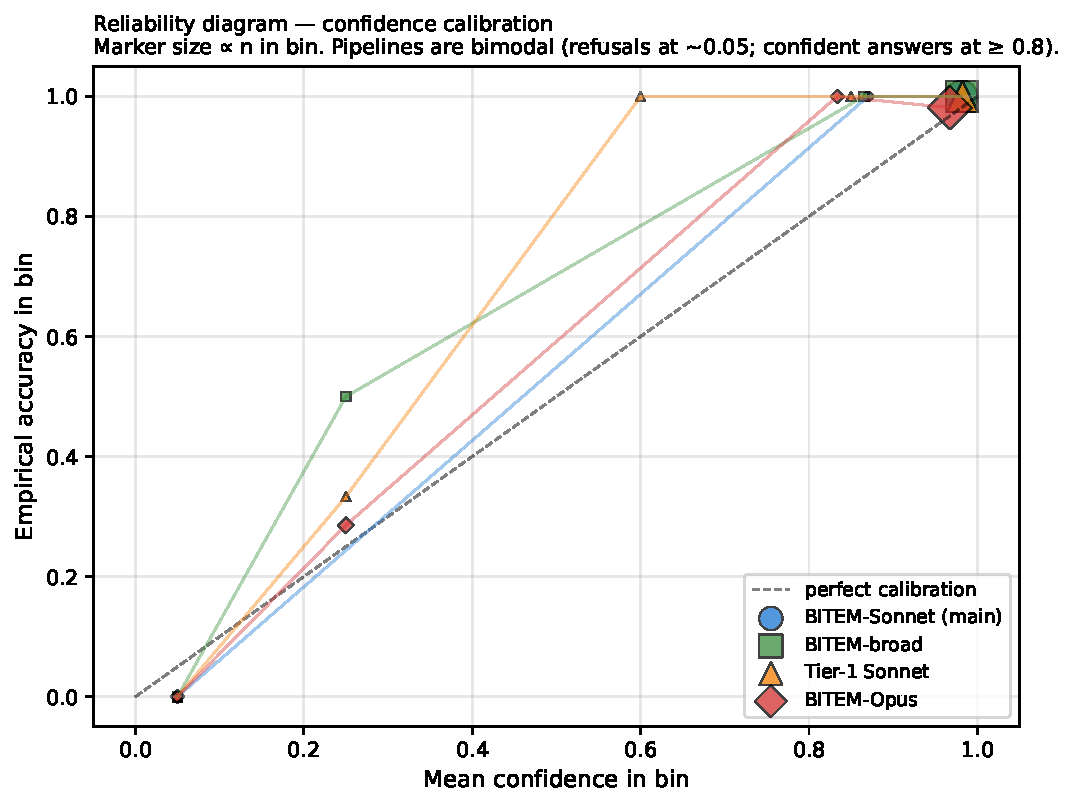
\includegraphics[height=0.70\textheight]{../figures/fig_reliability.pdf}
\par\vspace{0.3em}
{\small For AC-1, mean confidence 0.956 vs.\ accuracy 0.953 could hide poor per-bin reliability;
this diagram checks all submitted runs per bin (main system AC-2 highlighted).}
\end{frame}

\begin{frame}{Backup: the exact confidence rule}
\begin{itemize}\setlength\itemsep{0.5em}
  \item Verifier emits \texttt{match\_score} $\in\{0,1,2\}$ by re-deriving the answer
        from the entailed nuggets alone
  \item No entailed nuggets, or empty answer $\Rightarrow$ \textbf{refuse} (\texttt{conf}$=5$)
  \item \texttt{match\_score}$=0 \Rightarrow$ cap self-confidence at \textbf{25}
  \item \texttt{match\_score}$=1 \Rightarrow$ cap at \textbf{60}
  \item \texttt{match\_score}$=2 \Rightarrow$ leave unchanged
\end{itemize}
\vspace{0.6em}
{\small Abstention behaviour and configuration selected on val250 (248 synthetic topics);
the 65 official topics were never used for tuning.}
\end{frame}

\begin{frame}{Backup: limitations}
\begin{itemize}\setlength\itemsep{0.4em}
  \item LLM-judged ground truth throughout; none of it human-validated
  \item Self-evaluator validation is partly \textbf{in-sample}; the held-out
        cross-family check is weak ($\rho{=}0.60$, $n{=}5$, not significant)
  \item Synthetic tuning data is itself LLM-generated (Claude)
  \item Transfer and base-model swap are scored by a \textbf{surrogate judge}
  \item Model-tier ablations hold prompts fixed --- they measure naive substitution,
        not model capability
  \item $n=64$ topics. Significance is reported only for the \MNP{} lead; the \HMR{}
        and Accuracy leads and the $+$0.065 transfer mean are point estimates
\end{itemize}
\end{frame}

\end{document}
